\documentclass[conference]{IEEEtran}
\IEEEoverridecommandlockouts{}

\usepackage{cite}
\usepackage{amsmath,amssymb,amsfonts}
\usepackage{algorithmic}
\usepackage{graphicx}
\usepackage{textcomp}
\usepackage{xcolor}
\usepackage{tabularx, multirow}
\usepackage{float}
\usepackage{url}

\newcommand{\bolditalic}[1]{\textbf{\textit{#1}}}

% chktex-file 44

\def\BibTeX{{\rm B\kern-.05em{\sc i\kern-.025em b}\kern-.08em
    T\kern-.1667em\lower.7ex\hbox{E}\kern-.125emX}}
\begin{document}

\title{Programación lineal ejecutada con el método de Gauss-Seidel\\}

\author{\IEEEauthorblockN{1\textsuperscript{st} Mauro Alonso Gonzalez Figueroa}
    \IEEEauthorblockA{\textit{Universiddad Tecnologica de Bolivar} \\
        \textit{UBT}\\
        Cartagena, Colombia \\
        maugonzalez@utb.edu.co}
    \and
    \IEEEauthorblockN{2\textsuperscript{nd} German De Armas Castaño}
    \IEEEauthorblockA{\textit{Universidad Tecnologica de Bolivar} \\
        \textit{UTB}\\
        Cartagena, Colombia \\
        gdearmas@utb.edu.co}
    \and
    \IEEEauthorblockN{3\textsuperscript{rd} Angel Vega Rodriguez}
    \IEEEauthorblockA{\textit{Universidad Tecnologica de Bolivar} \\
        \textit{UTB}\\
        Cartagena, Colombia \\
        anvega@utb.edu.co}
}

\maketitle

\bibliographystyle{IEEETran}

\begin{abstract}
    In the realm of numerical analysis, the Gauss-Seidel method stands as an
    iterative technique employed to resolve systems of linear equations. It
    represents a refined version of the Jacobi method, often exhibiting
    superior convergence properties. Within the scope of this paper, we delve
    into the application of the Gauss-Seidel method to address a system of
    linear equations arising from a financial planning conundrum. Our
    endeavor demonstrates the efficacy and efficiency of the Gauss-Seidel
    method in tackling this type of system.
\end{abstract}

\begin{IEEEkeywords}
    Gauss-Seidel method, linear equations, financial planning
\end{IEEEkeywords}

\nocite{*}

\section{Introduction}
En el ámbito de la gestión empresarial, la Investigación de Operaciones
\textit{(IO)} se erige como una herramienta fundamental para la optimización de
procesos y la toma de decisiones estratégicas. Esta disciplina, basada
en el método científico y el análisis matemático, permite a las
organizaciones abordar problemas complejos de manera sistemática y
eficiente, conduciéndolas hacia el logro de sus objetivos.

En esencia, la IO se caracteriza por la aplicación de un enfoque
interdisciplinario que integra conocimientos de diversas áreas, como
las matemáticas, la estadística, la ingeniería y la economía. Este
enfoque colaborativo permite a los equipos de trabajo abordar problemas
complejos desde múltiples perspectivas, generando soluciones innovadoras
y efectivas.

\section{Gauss-Seidel}

Dentro del amplio arsenal de técnicas empleadas en la IO, el método
Gauss-Seidel se destaca como un algoritmo iterativo de gran utilidad para
la resolución de sistemas de ecuaciones lineales. Este método, ampliamente
reconocido por su simplicidad y eficiencia, se basa en la actualización
progresiva de las variables del sistema en función de las aproximaciones
más recientes de las demás. A través de un proceso iterativo, las
estimaciones se van refinando hasta alcanzar un punto de convergencia, donde
las soluciones satisfacen los criterios establecidos.

En el contexto de la programación lineal, el método Gauss-Seidel cobra
especial relevancia como herramienta complementaria al método simplex. Si
bien el método simplex se considera el enfoque tradicional para resolver
este tipo de problemas, el método Gauss-Seidel ofrece una alternativa viable
para abordar problemas de gran escala o aquellos con características
específicas que dificultan la aplicación del simplex.

\section{Marco Teorico}

\subsection{Programación lineal}

La programación lineal es una técnica de modelización matemática desarrollada
a partir de la década de 1930. Desde entonces, se ha aplicado con
frecuencia en los procesos de toma de decisión de numerosos ámbitos
económicos y productivos. La técnica de programación lineal proporciona
soluciones las soluciones abiertas \textit{(no son formulas estrictas ni
    nada por el estilo)}, que más bien se determinan mediante algoritmos.

\begin{figure}[H]
    \begin{center}
        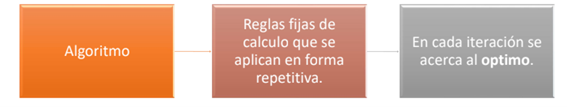
\includegraphics[width=\linewidth]{./Images/ProgramacionLineal.png}
        \caption{}
    \end{center}
\end{figure}

Algunos lineamientos generales para la implementación de la IO en la práctica.

\begin{enumerate}
    \item Definición del problemas
    \item Construcción del modelo
    \item Solución del modelo
    \item Validación del modelo
    \item implementación de la solución
\end{enumerate}

\subsection{Problema infactible}

Si no se encuentra ninguna solución que satisfaga todas las
restricciones del problema, el método simplex concluye que el problema
es infactible (No existe una solución que cumpla todas las
restricciones impuestas).

\subsection{Región factible}

Es el conjunto de todas las posibles soluciones que satisfacen todas las
restricciones del problema. Esta región es fundamental para entender la
naturaleza de las soluciones potenciales y para aplicar el método simplex
u otros algoritmos de optimización.

\subsubsection*{Características de la region factible}

\begin{enumerate}
    \item n un problema con dos variables, la región factible puede
          visualizarse como un área en el plano cartesiano. Con tres variables,
          sería un volumen en el espacio tridimensional, y con más variables, se
          representa en dimensiones superiores.

    \item La región factible es siempre una región convexa, lo que significa
          que cualquier combinación lineal de puntos dentro de la región también
          está dentro de la región.
\end{enumerate}


\subsection{Método o algebra simplex}

El Método Simplex es un método analítico de solución de problemas de
programación lineal capaz de resolver modelos complejos. Aunque es un
procedimiento algebraico, sus conceptos fundamentales son geométricos.
El Simplex es un método iterativo que permite ir mejorando la solución en
cada paso. El método consiste en caminar de vértice en vértice de manera que
aumente o disminuya la función objetivo (según el criterio). Si existe el
poliedro factible, el número de vértices que presenta es finito.

\begin{figure}[H]
    \begin{center}
        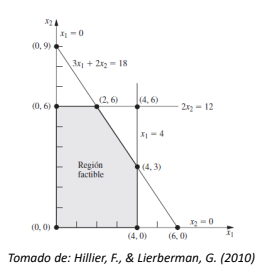
\includegraphics[width=.7\linewidth]{./Images/MetodoSimplex.png}
        \caption{}
    \end{center}
\end{figure}

\begin{figure}[H]
    \begin{center}
        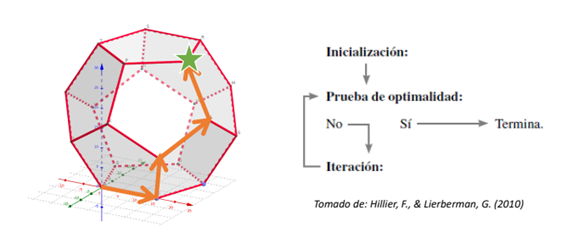
\includegraphics[width=\linewidth]{./Images/MetodoSimplex2.png}
        \caption{}
    \end{center}
\end{figure}

\subsection{Método de Gauss-Seidel}

Es un algoritmo utilizado para resolver sistemas de ecuaciones lineales. Es
una variante del método de relajación y es especialmente útil cuando se
trabaja con matrices grandes y densas.

En términos básicos, el método de Gauss-Seidel procede iterativamente,
actualizando cada variable de un sistema de ecuaciones en función de las
aproximaciones más recientes de las otras variables. En cada iteración, las
nuevas estimaciones se utilizan para mejorar las aproximaciones de las
variables restantes. Este proceso continúa hasta que las soluciones convergen
a un valor aceptable.

El método de Gauss-Seidel puede ser más eficiente computacionalmente que
otros métodos para resolver sistemas de ecuaciones lineales, especialmente
cuando se trata de sistemas que son diagonales dominantes o simétricos
positivos definidos. Sin embargo, su convergencia no está garantizada para
todos los sistemas, y puede ser lento o incluso divergente en algunos casos.
Por lo tanto, a veces se requieren ajustes o técnicas adicionales para
garantizar la convergencia adecuada.

\subsection{Vector gradiente}

También conocido como vector gradiente (denotado $\nabla$f), es un
campo vectorial que indica la dirección en la cual el campo f varía más
rápidamente y su módulo representa el ritmo de variación de f en la dirección
de dicho vector gradiente.

\begin{figure}[H]
    \begin{center}
        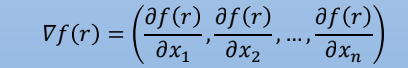
\includegraphics[width=\linewidth]{./Images/VectorGradiente.png}
        \caption{}
    \end{center}
\end{figure}

\subsection{Modelo estándar}

En el método simplex es una forma particular de formular un problema de
programación lineal que facilita su resolución mediante este método. Para
aplicar el método simplex, es necesario que el problema esté expresado en
términos de maximización con todas las restricciones como igualdades y todas
las variables no negativas.

\subsection{Variables Artificiales}

son variables adicionales introducidas en el problema para convertir
restricciones complicadas en una forma que permita aplicar el método
simplex. Estas variables no tienen significado en el contexto del problema
original, sino que son herramientas auxiliares para encontrar una
solución inicial.

\subsubsection*{¿Cuándo se utilizan las Variables Artificiales?}

Cuando una restricción es de igualdad (por ejemplo,
$a_{1}x_{1} + a_{2}x_{2} = b$), necesitamos una
variable artificial para iniciar el método simplex porque no podemos
simplemente añadir una variable de holgura (slack variable, esta variable
representa el espacio libre) como en las
restricciones $\leq$.

\subsubsection*{Restricciones de Desigualdad (del tipo $\leq$)}

Para una restricción del tipo ($a_{1}x_{1} + a_{2}x_{2} \leq b$), primero restamos una variable de
exceso (surplus variable) y luego añadimos una variable artificial para
convertirla en una ecuación de igualdad.

\subsection{Precio sombra}

El precio sombra puede representar una disposición a pagar por unidad
adicional de recurso. Si el precio del recurso es menor al precio sombra
entonces existirá un incentivo a ``comprar'' más debido a que esto tendrá un
impacto neto positivo en la función objetivo.

\section{Ejercicios propuestos}

\subsection{\textit{2Crudos Inc.}}

\subsubsection{Enunciado}

\textit{2Crudos Inc.} es una empresa petrolera que tiene una refinería en
la costa de Texas. La refinería procesa crudo proveniente de Arabia Saudita y
Venezuela, produciendo gasolina, diesel, y lubricantes.

Los dos crudos se diferencian en su composición química, por lo que
producen diferentes cantidades de cada producto. Un barril de crudo
proveniente de Arabia Saudita produce 0.3 barriles de gasolina, 0.4 barriles
de diesel, y 0.2 barriles de lubricantes. Por otro lado, un barril proveniente
de Venezuela produce 0.4 barriles de gasolina, 0.2 barriles de diesel, y
0.3 barriles de lubricantes. El restante 10\% del crudo se pierde en el
proceso de refinación. Los crudos también difieren en precio y
disponibilidad.~\textit{2Crudos Inc.} puede comprar a Arabia Saudita hasta 9000
barriles por día a un precio de \$20 por barril. Puede comprar a Venezuela
hasta 6000 barriles por día a un precio de \$15 por barril.

Los contratos establecidos por \textit{2Crudos Inc.} lo obligan a producir 2000
barriles diarios de gasolina, 1500 barriles diarios de diesel, y 500
barriles diarios de lubricantes ¿Como se pueden cumplir estos requerimientos
de la forma más eficiente?.

\subsubsection{Formulación matemática del problema}

\hfil{}

\textbf{Variables}

\begin{itemize}
    \item $X_{a} = $ Costo por barril comprado a Arabia Saudita
    \item $X_{v} = $ Costo por barril comprado en Venezuela
\end{itemize}

\textbf{Función objetivo}

\begin{equation*}
    \min Z = 20X_{a} + 15X_{v}
\end{equation*}

\textbf{Restricciones}

\begin{itemize}
    \item $X_{a} \leq 9000$ ``restricción de compra para Arabia Saudita''
    \item $X_{v} \leq 6000$ ``restricción de compra para Venezuela''
    \item $0.3X_{a} + 0.4X_{v} \geq 2000$ ``restricciones de producción''
    \item $0.4X_{a} + 0.2X_{v} \geq 1500$
    \item $0.2X_{a} + 0.3X_{v} \geq 500$
    \item $X_{a} + X_{v} \geq 0$ ``restricción de no negatividad''
\end{itemize}

\begin{figure}[H]
    \begin{center}
        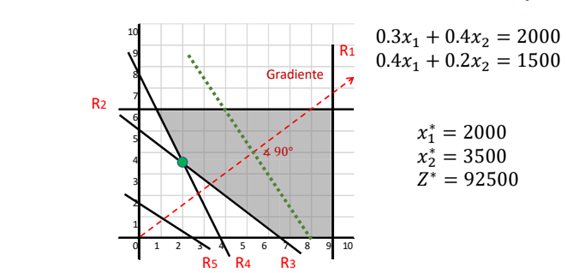
\includegraphics[width=\linewidth]{./Images/Caso-1_ImagenSolucion.png}
        \caption{}
    \end{center}
\end{figure}

Para garantizar la producción de barriles diaria 2 crudo inc debe comprar
2000 barriles provenientes de Arabia Saudita y 3500 de Venezuela, lo cual
tiene un costo de 92500 dólares.

\subsubsection{Justificacion}

Estudiar este tipo de problema es valioso por varias razones, tanto desde
una perspectiva académica como práctica bajo un contexto realista, ya que
permite analizar la eficiencia Operativa (cómo se pueden cumplir las
demandas de productos refinados de la manera más eficiente en términos
de costos), Aspectos Económicos (en cómo los precios de los insumos y
las restricciones de oferta llegan a afectan las decisiones de producción) e
incluso la toma de decisiones empresariales (gestión de recursos) y
análisis de sensibilidad (evaluar cómo cambios en los precios o en las
disponibilidades afectan las decisiones).

\subsection{\textit{Gutchi Company}}

\subsubsection{Enunciado}

Gutchi Company fabrica bolsos de mano, bolsos para rasuradora y mochilas. Para
elaborar los productos se necesita como materia prima piel animal. El proceso
de producción requiere dos tipos de mano de obra calificada: costura y
acabado. La siguiente tabla da la disponibilidad de los recursos, su
consumo por los tres productos y las utilidades por unidad.

\begin{table}[H]
    \begin{center}
        \begin{tabularx}{\linewidth}{ccccc}
            \multicolumn{5}{c}{Requerimientos de recursos por unidad}                                                     \\\hline

            \multirow{2}{*}{Recurso}                                                        &
            \multirow{2}{*}{\begin{tabular}{@{}c@{}}Bolsas \\ de Mano\end{tabular}}         &
            \multirow{2}{*}{\begin{tabular}{@{}c@{}}Bolsos para \\ rasuradora\end{tabular}} &
            \multirow{2}{*}{Mochilas}                                                       &
            \multirow{2}{*}{\begin{tabular}{@{}c@{}}Disponibilidad \\ diaria\end{tabular}}                                \\\\\hline

            \\

            Piel ($ft^{2}$)                                                                 & 2   & 26 & 3  & 24 $ft^{2}$ \\
            Costura ($h$)                                                                   & 2   & 1  & 2  & 40 $h$      \\
            Acabado ($h$)                                                                   & 1   & 5  & 20 & 45 $h$      \\\\\hline

            \\

            Precio de venta (\$)                                                            & 100 & 22 & 66               \\\\\hline
        \end{tabularx}
    \end{center}
\end{table}

\begin{equation*}
    \max Z = 100x_{1} + 22x_{2} + 66x_{3}
\end{equation*}

\subsubsection*{S.A}

\begin{align*}
    2x_{1} + 26x_{2} + 3x_{3} \leq 24 \\
    2x_{1} + x_{2} + 20x_{3} \leq 40  \\
    x_{1} + 0.5x_{2} + x_{3} \leq 45
\end{align*}

\begin{align*}
    x_{1}, x_{2}, x_{3} \geq 0
\end{align*}

\subsection*{Forma estándar}

\begin{equation*}
    \max Z = 100x_{1} + 22x_{2} + 66x_{3}
\end{equation*}

\subsubsection*{S.A}

\begin{align*}
    2x_{1} + 26x_{2} + 3x_{3} + s_{1} \leq 24 \\
    2x_{1} + x_{2} + 20x_{3}  + s_{2} \leq 40 \\
    x_{1} + 0.5x_{2} + x_{3}  + s_{3} \leq 45
\end{align*}

\begin{align*}
    x_{1}, x_{2}, x_{3}, s_{1}, s_{2}, s_{3} \geq 0
\end{align*}

\subsubsection*{Procedimiento}

La formulación del problema en primera instancia se resuelve igual
que con el anterior método, pero para su solución se deben transformar
las ecuaciones a su forma estándar ya que garantiza la uniformidad,
simplicidad y optimalidad del método simplex, conservando la función
objetivo y asegurando que todas las variables sean no negativas.

Debido a las similitudes que tiene el método simplex con el método
algebraico de Gauss-Seidel (basados en iteraciones), implementamos dicho
método para dar respuesta a las incógnitas planteadas en el problema.

\begin{itemize}
    \item $x_{1} = 8.75$
    \item $x_{2} = 9.67$
    \item $x_{3} = 8.85$
    \item $s_{1} = 0.26$
    \item $s_{2} = 3.00$
    \item $s_{3} = 21.0$
\end{itemize}

Dándonos como resultado que para maximizar el costo por unidad vendida y
fabricada, por \textit{Gutchi Co.} se deben producir $8.75$ bolsos de mano,
$9.67$ bolsos para rasuradora, y $8.85$ mochilas (los valores decimales
se asocian a los productos que están en proceso o que directamente
no están terminados), dando como resultado una ganancia de $\$1006.84$ por
la venta de los tres productos.

Ademas por la naturaleza del método Gauss-Seidel, el programa nos proporciona
el valor de las variables de holgura o lo que seria lo mismo, a la cantidad
que se desplazaría en inventarios, lo cual, los convierte en materia
prima utilizable para un nuevo ciclo.

\begin{itemize}
    \item Materiales de inventario de bolsos de mano: $0.26$
    \item Materiales de inventario de bolsos para rasuradora: $3.00$
    \item Materiales de inventario para mochilas: $21.0$
\end{itemize}

\bibliography{./Bibliography/bibliography.bib}

\end{document}
